%!TeX root=../tese.tex
%("dica" para o editor de texto: este arquivo é parte de um documento maior)
% para saber mais: https://tex.stackexchange.com/q/78101

%!TeX root=../tese.tex
%("dica" para o editor de texto: este arquivo é parte de um documento maior)
% para saber mais: https://tex.stackexchange.com/q/78101

\chapter{Conexidade em grafos dinâmicos}

\enlargethispage{.8\baselineskip}

\section{Definição}
\label{sec:definition}

Como citado no Capítulo~1, o problema da conexidade em grafos dinâmicos visa construir um algoritmo eficiente que dá suporte a inserções, remoções e consultas de conexidade. O algoritmo de Holm, de Lichtenberg e Thorup~\cite{jacob_holm} para este problema de conexidade é composto por $\left\lceil \lg n \right\rceil$ florestas dinâmicas do grafo $G$, e utiliza uma biblioteca que será descrita na Subseção 2.2. 

\section{Conexidade em florestas dinâmicas}
\label{sec:dynamic-forest-connectivity}

Rodrigues \cite{arthur}, em sua dissertação do mestrado, estudou, entre outros assuntos, o problema da conexidade em florestas dinâmicas e implementou o seu algoritmo, que foi proposto na Seção~2 do artigo de Holm, de Lichtenberg e Thorup~\cite{jacob_holm}. No Capítulo~2 da sua dissertação ele descreve as rotinas principais do algoritmo, baseado em \textit{Euler tour trees}, e realiza uma análise minuciosa da complexidade de tempo das funções dos pseudocódigos. Dada essas circunstâncias, optamos por não apresentar uma descrição detalhada desse algoritmo, explicando brevemente sobre o que as rotinas principais fazem, bem como algumas diferenças da nossa implementação em código comparadas com a de Rodrigues.  

O problema da conexidade em florestas dinâmicas pode ser considerada uma simplificação do problema de conexidade em grafos dinâmicos, quando o grafo em questão é uma floresta. A biblioteca que usaremos contém os seguintes métodos:

\begin{itemize}
    \item \texttt{\textbf{florestaDinâmica(F, n)}}: constrói e devolve uma floresta dinâmica $F$ com $n$ vértices isolados;
    \item \texttt{\textbf{conectadosFD(F, u, v)}}: devolve verdadeiro se \textit{u} e \textit{v} estão na mesma componente da floresta $F$ e falso caso contrário;
    \item \texttt{\textbf{adicioneFD(F, u, v)}}: insere uma aresta \textit{uv} na floresta $F$;
    \item \texttt{\textbf{removaFD(u, v)}}: remove a aresta \textit{uv} da floresta $F$;
\end{itemize}

A estrutura de dados principal usada neste algoritmo de Holm, de Lichtenberg e Thorup~para dar suporte eficientes às rotinas acima é uma árvore binária de busca balanceada (ABBB). Dessa forma, a floresta dinâmica é constituída de várias ABBBs. Rodrigues utiliza \textit{treaps} em sua implementação, que é de natureza aleatória. Em nosso caso, utilizamos árvores \textit{splay}, que foram desenvolvidas por \textit{Sleator e Tarjan} \cite{sleator}. Árvores \textit{splay} são árvores binárias de busca (ABBs) que possuem uma rotina extra (além das usuais de busca, inserção e remoção) chamada \textit{splay}, que é acionada ao final de cada operação feita na árvore, de modo que é sempre aplicada ao nó mais profundo visitado. Isso faz com que o custo amortizado da operação \textit{splay} seja $O(\lg n)$, onde $n$ é o número de nós da árvore, e que também uma sequência de $m$ acessos em uma árvore \textit{splay} tenha custo total $O(m \lg n)$.  Como também já existe bastante literatura sobre árvores \textit{splay}, e seu funcionamento interno não afeta a descrição dos algoritmos que descreveremos, não entraremos em detalhes de sua implementação.

\section{Estrutura do grafo dinâmico}
\label{sec:dynamic-graph-structure}

Para implementar o grafo dinâmico, resume-se à construção da seguinte biblioteca de forma eficiente:

\begin{itemize}
    \item \texttt{\textbf{grafoDinâmico(G, n)}}: contrói e devolve um grafo dinâmico $G$ com $n$ vértices isolados;
    \item \texttt{\textbf{conectadosGD(G, u, v)}}: devolve verdadeiro se os vértices $u$ e $v$ estão na mesma componente de $G$ e falso caso contrário;
    \item \texttt{\textbf{adicioneGD(G, u, v)}}: adiciona a aresta $uv$ no grafo $G$;
    \item \texttt{\textbf{removaGD(G, u, v)}}: remove a aresta $uv$ do grafo $G$.
\end{itemize} 

Nossa implementação encapsula a complexidade de manutenção de $\left\lceil \lg n \right\rceil$ florestas dinâmicas em uma abstração do grafo dinâmico. 
Assim, a consulta \texttt{conectadosGD} aplicada ao grafo $G$ significa fazer a mesma consulta para alguma floresta maximal $F$ de $G$. Dessa maneira, sempre que estivermos realizando alguma operação de alteração ou consulta de conexidade em nosso grafo $G$, estamos também a realizando em uma floresta dinâmica $F$ que seja maximal em $G$. Da mesma forma, quando chamamos o construtor do grafo dinâmico, estamos criando $\left\lceil \lg n \right\rceil$ florestas de vértices isolados.

\section{Adição de arestas no grafo dinâmico}
\label{sec:dynamic-graph-edge-addition}

Quando realizamos uma chamada à função \texttt{adicioneGD}, é feita uma chamada ao \texttt{conectadosGD} para verificar a conexidade de $u$ com $v$ em $G$. Se estes vértices não estiverem ligados em $G$, então é inserido a aresta $uv$ na floresta maximal que estamos mantendo, assim ligando a árvore que contém $u$ com a que contém $v$ nessa floresta. Chamamos essas arestas de \textbf{arestas da floresta}.

Caso $u$ e $v$ já estiverem conectados em $G$, então essa aresta $uv$ é chamada de \textbf{aresta reserva} e ela será armazenada em um grafo representado por listas de adjacências, que contém a seguinte biblioteca:

\begin{itemize}
    \item \texttt{\textbf{listaDeAdjacências(L, n)}}: constrói e devolve um grafo $L$ contendo $n$ listas de adjacências, onde $n$ é o número de vértices isolados;
    \item \texttt{\textbf{adicioneLA(L, u, v)}}: adiciona $u$ na lista de adjacências de v em $L$ e vice-versa;
    \item \texttt{\textbf{removaLA(L, u, v)}}: remove $u$ da lista de adjacências de $v$ em $L$ e vice-versa.
\end{itemize} 

A nossa implementação \cite{chung2025} para lista de adjancências possui um custo O($n$) ao acionar o construtor \texttt{listaDeAdjacências}, e para 
as rotinas \texttt{adicioneLA} e \texttt{removaLA} são garantidos o tempo esperado O($1$) visto que estamos utilizando um mapa hash da linguagem \textit{C++} para realizar adição de um vizinho $v$ em $u$ e, se houver, remoção de $v$ da lista de adjancência de $u$.

Como a inserção de arestas (\texttt{adicioneFA}) em uma floresta dinâmica com $n$ vértices possui uma complexidade de tempo esperado O(lg$n$), então temos que \texttt{adicioneGD} também terá o seu custo esperado de tempo O(lg$n$). 

O objetivo de guardar arestas reservas em nosso grafo é simples. Seja o grafo $G$ com $V = \{a, b, c, d, e, f, g\}$ e suas respectivas arestas, como ilustrado na Figura~\ref{fig:graph_without_reserve_edges}. Temos dois subgrafos $G_1$ e $G_2$ em nosso grafo $G$. O vértice $a$ está em $G_1$ e $e$ está em $G_2$. Se $G_1$ e $G_2$ são conectados por uma única aresta $ae$, a remoção dela acarretaria em duas componentes separadas. Então chamar \texttt{conectados(G, a, e)} após a remoção de $ae$ receberíamos falso como resposta. 

\begin{figure}
    \centering
    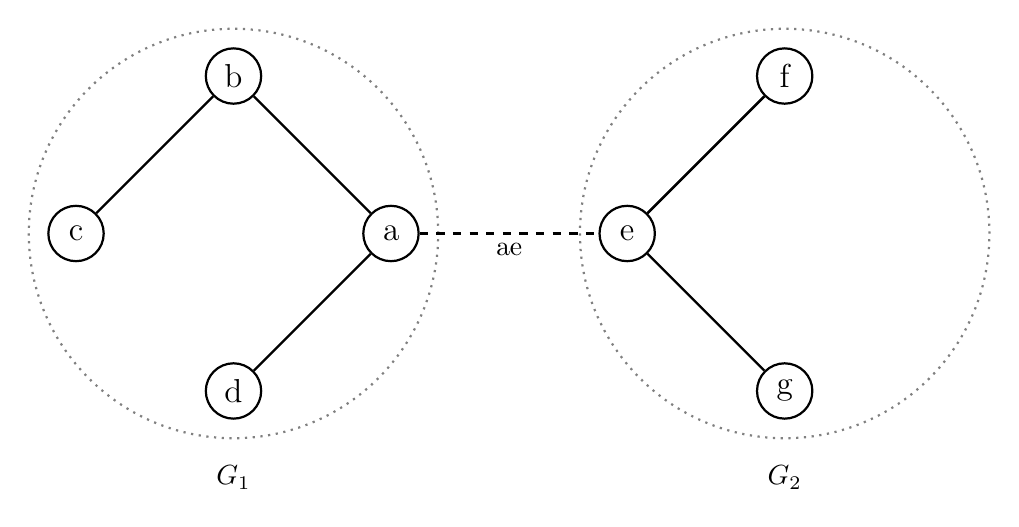
\begin{tikzpicture}
        [node/.style={circle,draw,minimum size=2em, thick, font=\large},
        edge/.style={thick, black},
        reserve/.style={red, very thick, dashed},
        removed/.style={black, thick, dashed}]

        % Vertices in a circular arrangement
        \node[node] (a) at (-1,2) {a};
        \node[node] (b) at (-3,4) {b};
        \node[node] (c) at (-5,2) {c};
        \node[node] (d) at (-3,0) {d};
        \node[node] (e) at (2,2) {e};
        \node[node] (f) at (4,4) {f};
        \node[node] (g) at (4,0) {g};
        
         % Dotted circles for T_u and T_v
        \draw[dotted, thick, gray] (-3,2) circle (2.6cm); % T_u circle around {a,b,c,d}
        \draw[dotted, thick, gray] (4,2) circle (2.6cm);  % T_v circle around {e,f,g}
        
        % Labels for the circles
        \node at (-3,-1.1) {$G_1$};
        \node at (4,-1.1) {$G_2$};


        % tree edges (normal black edges)
        \draw[edge] (a) -- (b) node[midway, below] {};
        \draw[edge] (b) -- (c) node[midway, below] {};
        \draw[edge] (a) -- (d) node[midway, below] {};
        \draw[edge] (e) -- (f) node[midway, below] {};
        \draw[edge] (e) -- (f) node[midway, below] {};
        \draw[edge] (e) -- (g) node[midway, below] {};
        \draw[removed] (a) -- (e) node[midway, below] {ae};

        % MST edges ( in red)
        %\draw[reserve] (d) -- (g) node[midway, below] {dg};
        
    \end{tikzpicture}
    \caption{Um grafo com sete vértices e sem nenhuma aresta reserva. O subgrafo $G_1$ contém os vértices $a$, $b$, $c$ e $d$, enquanto $G_2$ contém os vértices $e$, $f$ e $g$. A aresta tracejada $ae$ está prestes a ser removida.}
    \label{fig:graph_without_reserve_edges}
\end{figure}

Agora, suponha que $G_1$ e $G_2$ eram componentes conexas separadas, e foram  conectadas pela aresta $ae$, tornando-se uma única componente conexa, como mostra a Figura~\ref{fig:graph_with_reserve_edges}. Ao chamarmos \texttt{adiciona(G, d, g)}, guardaríamos a aresta $dg$ como reserva. Se posteriormente removermos $ae$, note que os subgrafos $G_1$ e $G_2$ estariam em duas componentes separadas. Assim, se não tivéssemos armazenado $dg$, então a consulta \texttt{conectados(G, a, e)} devolveria falso, o que estaria incorreto visto que a aresta $dg$ existe de fato no grafo. Dessa forma, a aresta reserva possui a função de substituir a aresta removida, como veremos adiante, mantendo a conexão entre $G_1$ e $G_2$.

\begin{figure}
    \centering
    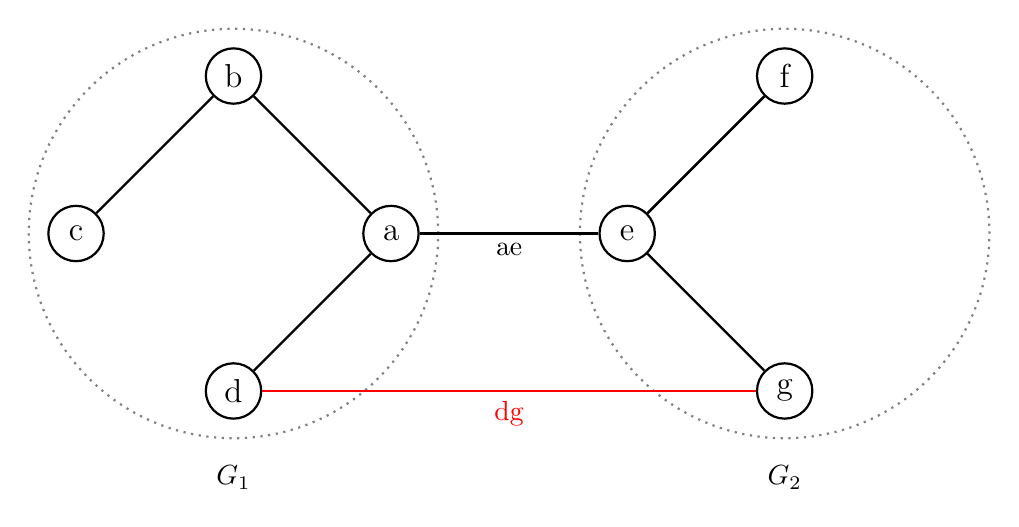
\begin{tikzpicture}
        [node/.style={circle,draw,minimum size=2em, thick, font=\large},
        edge/.style={thick, black},
        reserve/.style={red, thick},
        removed/.style={black, thick, dashed}]

        % Vertices in a circular arrangement
        \node[node] (a) at (-1,2) {a};
        \node[node] (b) at (-3,4) {b};
        \node[node] (c) at (-5,2) {c};
        \node[node] (d) at (-3,0) {d};
        \node[node] (e) at (2,2) {e};
        \node[node] (f) at (4,4) {f};
        \node[node] (g) at (4,0) {g};
        
         % Dotted circles for T_u and T_v
        \draw[dotted, thick, gray] (-3,2) circle (2.6cm); % T_u circle around {a,b,c,d}
        \draw[dotted, thick, gray] (4,2) circle (2.6cm);  % T_v circle around {e,f,g}
        
        % Labels for the circles
        \node at (-3,-1.1) {$G_1$};
        \node at (4,-1.1) {$G_2$};


        % tree edges (normal black edges)
        \draw[edge] (a) -- (b) node[midway, below] {};
        \draw[edge] (b) -- (c) node[midway, below] {};
        \draw[edge] (a) -- (d) node[midway, below] {};
        \draw[edge] (e) -- (f) node[midway, below] {};
        \draw[edge] (e) -- (f) node[midway, below] {};
        \draw[edge] (e) -- (g) node[midway, below] {};
        \draw[edge] (a) -- (e) node[midway, below] {ae};

        % MST edges ( in red)
        \draw[reserve] (d) -- (g) node[midway, below] {dg};
        
    \end{tikzpicture}
    \caption{Um grafo com sete vértices. O subgrafo $G_1$ contém os vértices $a$, $b$, $c$ e $d$, enquanto $G_2$ contém os vértices $e$, $f$ e $g$. A aresta vermelha $dg$ é uma aresta reserva do grafo.}
    \label{fig:graph_with_reserve_edges}
\end{figure}

Note que não podemos simplesmente adicionar $dg$ como aresta da floresta maximal de $G$ em vez de guardar nas listas de adjacências. Como por definição uma floresta não pode conter ciclos, adicionar $dg$ dada a existência da aresta $ae$ acarretaria na formação de um ciclo contendo essas duas arestas, o que violaria a estrutura do algoritmo, já que queremos manter árvores binárias de busca balanceadas para garantir a complexidade de tempo logarítmica em suas rotinas. Como um grafo pode conter ciclos, guardar a aresta como reserva é uma forma de manter o grafo correto e o algoritmo eficiente. 

\section{Remoção de arestas no grafo dinâmico}
\label{sec:dynamic-graph-edge-removal}

Dessa forma, quando queremos remover uma aresta reserva, podemos simplesmente acionar a rotina \texttt{removaLA} (da lista de adjacências) e a floresta maximal do grafo não será afetada. Entretanto, se queremos remover uma aresta $uv$ do grafo $G$, a floresta é quebrada em duas componentes, que podemos chamar de árvores $T_u$ e $T_v$, de modo que o primeiro contém o vértice $u$ e o segundo contém o vértice $v$. Dessa forma, precisamos verificar se existe alguma aresta reserva que liga $T_u$ a $T_v$, para que possamos garantir que o teste de conexidade de $u$ e $v$ esteja correto. Assim, precisamos procurar uma aresta reserva que irá substituir a aresta que foi removida de $G$, que vamos chamar de \textbf{aresta substituta}.

Podemos supor, sem perda de generalidade, que $|T_u| \leq |T_v|$, ou seja, o número de vértices de $T_u$ é no máximo o de $T_v$. Assim, para procurar uma aresta reserva que substitua a removida, precisaríamos percorrer cada vértice $x$ de $T_u$ e verificar se existe algum vértice $y$ na lista de adjacências de $x$, de modo que $y$ esteja em $T_v$. Se $y \in V(T_v)$, teríamos encontrado uma aresta substituta $xy$, bastando apenas acionar \texttt{adicioneGD(G, x, y)} para conectar os dois vértices e, consequentemente, $T_u$ e $T_v$ virariam uma única componente da floresta.

\begin{figure}
    \centering
    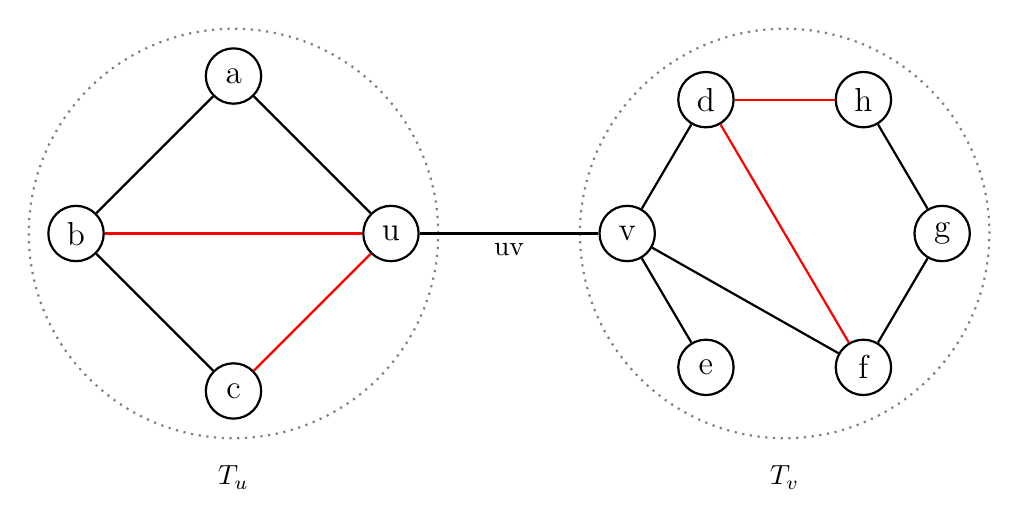
\begin{tikzpicture}
        [node/.style={circle,draw,minimum size=2em, thick, font=\large},
        edge/.style={thick, black},
        reserve/.style={red, thick},
        removed/.style={black, thick, dashed}]

        \node[node] (u) at (-1,2) {u};
        \node[node] (a) at (-3,4) {a};
        \node[node] (b) at (-5,2) {b};
        \node[node] (c) at (-3,0) {c};
        \node[node] (v) at (2,2) {v};
        \node[node] (d) at (3,3.7) {d};
        \node[node] (e) at (3,0.3) {e};
        \node[node] (f) at (5,0.3) {f};
        \node[node] (g) at (6, 2) {g};
        \node[node] (h) at (5, 3.7) {h};
        
        
         % Dotted circles for T_u and T_v
        \draw[dotted, thick, gray] (-3,2) circle (2.6cm);
        \draw[dotted, thick, gray] (4,2) circle (2.6cm);  
        
        % Labels for the circles
        \node at (-3,-1.1) {$T_u$};
        \node at (4,-1.1) {$T_v$};

        % tree edges (normal black edges)
        \draw[edge] (a) -- (u) node[midway, below] {};
        \draw[edge] (a) -- (b) node[midway, below] {};
        \draw[edge] (b) -- (c) node[midway, below] {};
        \draw[edge] (v) -- (d) node[midway, below] {};
        \draw[edge] (v) -- (f) node[midway, below] {};
        \draw[edge] (v) -- (e) node[midway, below] {};
        \draw[edge] (u) -- (v) node[midway, below] {uv};
        \draw[edge] (f) -- (g) node[midway, below] {};
        \draw[edge] (g) -- (h) node[midway, below] {};

        % reserve edges (normal red edges)
        \draw[reserve] (b) -- (u) node[midway, below] {};
        \draw[reserve] (c) -- (u) node[midway, below] {};
        \draw[reserve] (d) -- (f) node[midway, below] {};
        \draw[reserve] (d) -- (h) node[midway, below] {};

    \end{tikzpicture}
    \caption{Um grafo com 10 vértices. As arestas pretas são da floresta maximal do grafo, enquanto as vermelhas são arestas reservas.}
    \label{fig:graph_with_Tu_and_Tv}
\end{figure}

\newpage

Após a remoção da aresta $uv$, note que teremos duas componentes do grafo $G$ separadas em $T_u$ e $T_v$. Na Figura~\ref{fig:graph_with_Tu_and_Tv}, por exemplo, não temos uma aresta reserva que ligue $T_u$ e $T_v$. Sob essas condições, para achar uma aresta substituta precisamos percorrer cada vértice $a$ de $T_u$, e para cada vizinho $b$ de $a$ teríamos que verificar se $b \in V(T_v)$. Assim, o consumo de tempo esperado para essa busca exaustiva é de O($n^2$), visto que supusemos que não há nenhuma aresta reserva que ligue $T_u$ e $T_v$. Como \texttt{conectadosGD} tem consumo de tempo esperado O(lg$n$), então teremos um consumo de O($n^2$lg$n$) para \texttt{removaGD}, pois precisamos verificar se as duas pontas de cada aresta reserva estão conectadas chamando a rotina \texttt{conectadosGD}. Note que achamos uma aresta substituta caso as duas pontas da aresta reserva não estejam conectadas, pois uma delas estará em $T_u$ e outra estará em $T_v$.

Assim, torna-se necessário uma implementação mais eficiente para a rotina de remoção de arestas, e por isso apresentaremos a solução de Holm, de Lichtenberg e Thorup~\cite{jacob_holm}, que resolve este problema em O(lg$^2n$).

\begin{figure}
    \centering
    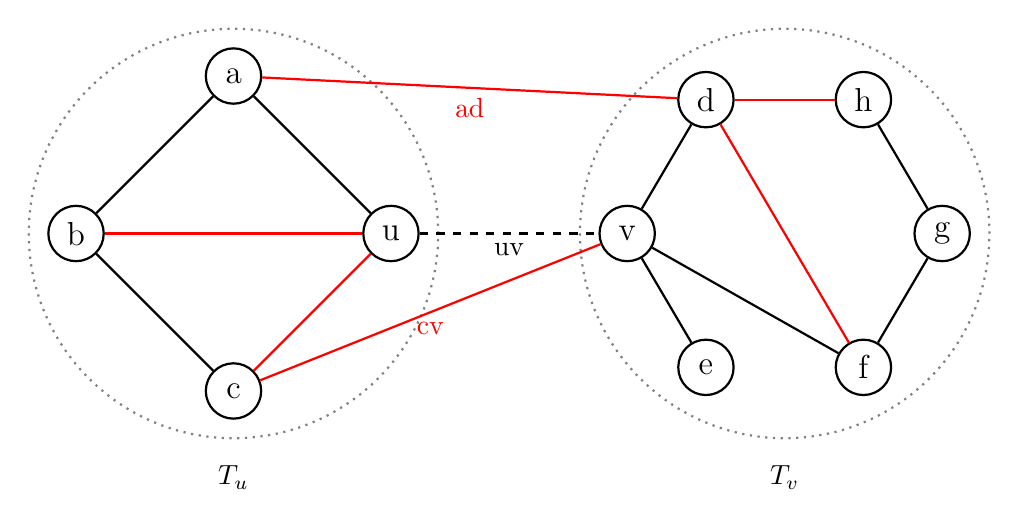
\begin{tikzpicture}
        [node/.style={circle,draw,minimum size=2em, thick, font=\large},
        edge/.style={thick, black},
        reserve/.style={red, thick},
        removed/.style={black, thick, dashed}]

        \node[node] (u) at (-1,2) {u};
        \node[node] (a) at (-3,4) {a};
        \node[node] (b) at (-5,2) {b};
        \node[node] (c) at (-3,0) {c};
        \node[node] (v) at (2,2) {v};
        \node[node] (d) at (3,3.7) {d};
        \node[node] (e) at (3,0.3) {e};
        \node[node] (f) at (5,0.3) {f};
        \node[node] (g) at (6, 2) {g};
        \node[node] (h) at (5, 3.7) {h};
        
        
         % Dotted circles for T_u and T_v
        \draw[dotted, thick, gray] (-3,2) circle (2.6cm);
        \draw[dotted, thick, gray] (4,2) circle (2.6cm);  
        
        % Labels for the circles
        \node at (-3,-1.1) {$T_u$};
        \node at (4,-1.1) {$T_v$};

        % tree edges (normal black edges)
        \draw[edge] (a) -- (u) node[midway, below] {};
        \draw[edge] (a) -- (b) node[midway, below] {};
        \draw[edge] (b) -- (c) node[midway, below] {};
        \draw[edge] (v) -- (d) node[midway, below] {};
        \draw[edge] (v) -- (f) node[midway, below] {};
        \draw[edge] (v) -- (e) node[midway, below] {};
        \draw[removed] (u) -- (v) node[midway, below] {uv};
        \draw[edge] (f) -- (g) node[midway, below] {};
        \draw[edge] (g) -- (h) node[midway, below] {};
        \draw[reserve] (a) -- (d) node[midway, below] {ad};
        \draw[reserve] (c) -- (v) node[midway, below] {cv};

        % reserve edges (normal red edges)
        \draw[reserve] (b) -- (u) node[midway, below] {};
        \draw[reserve] (c) -- (u) node[midway, below] {};
        \draw[reserve] (d) -- (f) node[midway, below] {};
        \draw[reserve] (d) -- (h) node[midway, below] {};

    \end{tikzpicture}
    \caption{As arestas pretas são da floresta maximal do grafo, enquanto as vermelhas são reservas. A aresta $uv$ tracejada está prestes a ser removida e substituída pela $ad$ ou $cv$, que ligam $T_u$ e $T_v$.}
    \label{fig:graph_with_Tu_and_Tv_with_reserve_edge}
\end{figure}

\newpage

\section{Fatiamento do grafo em níveis}
\label{sec:level-slicing}

Na Seção~3.1 do artigo de Holm, de Lichtenberg e Thorup~\cite{jacob_holm}, é apresentada essa técnica de fatiar o grafo em níveis. Cada aresta do grafo possui um nível entre $1$ e $\left\lceil \lg n \right\rceil$, onde $n$ é o número de vértices do grafo $G$. Toda vez que inserimos uma aresta em $G$, ela possuirá o nível $\left\lceil \lg n \right\rceil$, e ele nunca será aumentado. Assim, o nível da aresta somente será decrementado quando estamos buscando uma aresta substituta. 

Se $G$ é um grafo e $\emptyset \neq X \subseteq V(G)$, então o subgrafo de $G$ \textbf{induzido} ou \textbf{gerado} por $X$ é subgrafo $H$ de $G$ de modo que $V(H) = X$ e $E(H)$ é exatamente o conjunto de arestas de $G$ que têm ambos os extremos em $X$. Assim, podemos denotar $H$ como $G[X]$.

Sendo assim, podemos definir um grafo $G_i$, que é o grafo induzido pelas arestas de nível menor ou igual a $i$. Para cada nível $i$, iremos manter uma floresta maximal $F_i$ de $G_i$ e o grafo $L_i$, mantido como listas de adjacências que guardam apenas arestas reservas de nível $i$. Dessa forma, temos que $G_1 \subseteq G_2 \subseteq \cdots \subseteq G_{l_{max}} = G$, onde $l_{max} =  \left\lceil \lg n \right\rceil$, para um grafo de $n$ vértices. Consequentemente, temos que $F_{l_{max}}$ é uma floresta maximal de $G$. 

Assim, podemos estabelecer algumas invariantes, que são mantidas ao longo das modificações no grafo $G$:

\begin{enumerate}[label=(\Roman*)]
    \item \label{invariant1} $F_i$ é uma floresta maximal de $G_i$ para todo $1 \leq i \leq  \left\lceil \lg n \right\rceil$;
    
    \item \label{invariant2} $F_i \subseteq F_{i+1}$ para todo $1 \leq i \leq \left\lceil \lg n \right\rceil - 1$;
    
    \item \label{invariant3} Cada floresta $F_i$ possui no máximo $2^i$ vértices.
\end{enumerate}

O objetivo de fatiar o grafo em  $\left\lceil \lg n \right\rceil$ níveis é para caso uma aresta da floresta de nível $i$ for removida, não será mais necessário procurar exaustivamente por substitutas nos níveis menores que $i$. Assim, passamos a buscar a substituta inicialmente nas arestas reservas em $L_i$. Caso não a encontremos, passamos a procurar nas listas de adjacência $L_{i+1}, L_{i+2}, \ldots, L_{ \left\lceil \lg n \right\rceil}$. Se não existir uma aresta substituta em $R_j$, $i \leq j \leq  \left\lceil \lg n \right\rceil$, então rebaixaremos as arestas que exploramos em $R_j$ para um nível inferior $j-1$, caso $j > 0$. Tudo isso será retomado na seção seguinte, onde iremos detalhar mais nas implementações dos métodos principais da biblioteca do grafo dinâmico. 

\section{Implementação do grafo dinâmico}
\label{sec:dynamic-graph-implementation}

\subsection{Construtor}
\label{sec:code-constructor}

Para implementar um grafo dinâmico, chamamos \texttt{novoGD(n)} para inicializar cada $F_i$ e $L_i$ do grafo $G$ de $n$ vértices, $1 \leq i \leq \left\lceil \lg n \right\rceil$, chamando os métodos \texttt{novaFD(n)} e \texttt{novaLA(n)}, respectivamente. Isso quer dizer que estamos criando florestas dinâmicas e listas de adjacência com $n$ vértices isolados para cada nível $i$. Note que $F_{\left\lceil \lg n \right\rceil}$ e $L_{\left\lceil \lg n \right\rceil}$ representam o grafo dinâmico vazio, sem nenhuma aresta. 

Além disso, usamos um mapa hash para guardar e obter o nível de uma aresta $uv$ em tempo esperado O($1$). Assim, este mapa usa como chave os valores das pontas da aresta ($u$ e $v$) e retornam o valor do nível da aresta $uv$. Assim, podemos definir um outro método \texttt{novoMapaHash(n)} que devolve um mapa hash vazio para um grafo de $n$ vértices. Dessa forma, se chamarmos esse método e atribuir a uma variável chamada \textit{nível}, podemos realizar as seguintes operações com \textit{nível}:

\begin{itemize}
    \item \textit{nível[u, v]} $\leftarrow$ i: atribui o nível $i$ a uma aresta $uv$. 
    
    \item \textit{nível[u, v]} $\leftarrow$ \texttt{NIL}: remove a aresta $uv$ e, consequentemente, o seu nível.
    
    \item $x$ $\leftarrow$ \textit{nível[u, v]}: atribui o valor do nível da aresta $uv$ à variável $x$. 
\end{itemize}


Dessa forma, podemos enunciar o construtor do grafo no Programa~\ref{prog:newGD}. 

\begin{programruledcaption}{\texttt{novoGD(n)} \label{prog:newGD}}
    \noindent\textbf{Entrada}: Recebe um número $n$ de vértices do grafo. \\
    \textbf{Saída}: Devolve um grafo dinâmico $G$ com $n$ vértices isolados.
    \vspace{-0.5\baselineskip}
    \begin{lstlisting}[
        language={[brazilian]pseudocode},
        style=pseudocode,
        style=wider,
        functions={},
        specialidentifiers={},
        escapeinside={(*@}{@*)},
    ]
    \textbf{para} $i$ := $1$ \textbf{até} $\left\lceil \lg n \right\rceil$ \textbf{faça}
        G.$F_i$ := \texttt{novaFD(n)}
        G.$L_i$ := \texttt{novaLA(n)}
    G.nível := \texttt{novoMapaHash(n)}
    devolva G
    \end{lstlisting}
    \vspace{-0.5\baselineskip}
\end{programruledcaption}

Como ambos \texttt{novaFD(n)} e \texttt{novaLA(n)} consomem tempo O($n$), então \texttt{novoGD(n)} consome tempo O($n$lg$n$), pois estamos criando $\left\lceil \lg n \right\rceil$ florestas dinâmicas e listas de adjacências. Além, disso, as invariantes são mantidas porque estamos criando um grafo com $n$ vértices isolados.

\subsection{Nós do grafo}
\label{sec:graph-nodes}

Como adotamos a técnica de \textit{Euler tour trees} na implementação das nossas florestas dinâmicas, mencionada brevemente na Seção~\ref{sec:dynamic-graph-structure}, estamos utilizando uma estrutura chamada \textbf{nó} que armazena vários atributos relevantes, cuja funcionalidade será descrita mais detalhadamente nas Seções~\ref{sec:code-edge-addition} e \ref{sec:code-edge-removal}. 

Um nó pode representar tanto um vértice da forma $uu$ quanto uma aresta da forma $uv$, $u \neq v$. Assim, exclusivamente para cada nó do tipo aresta $uv$, iremos armazenar um atributo booleano chamado \textit{éNível}, que indica se tal aresta pertence a uma floresta maximal de nível $i$. Dessa forma, se $uv$ possui nível $2$, então em $F_2$ esse booleano será verdadeiro, e falso em outras $F_i$, $i \neq 2$. Além disso, iremos adicionar um contador \text{arestasDeNível} para cada nó do tipo aresta, a fim de calcular a quantidade de arestas em sua subárvore que tenham o booleano \textit{éNível} como verdadeiro. 

Já para o nó do tipo vértice $uu$, iremos armazenar um booleano chamado \textit{incideArestaReservaDeNível} que indica se $uu$ é uma das pontas de alguma aresta reserva com o booleano \textit{éNível} verdadeiro. Dessa forma, se $uv$ é aresta reserva e possui nível $2$, então os vértices $u$ e $v$ em $F_2$ terão \textit{incideArestaReservaDeNível} como verdadeiro. Além disso, iremos manter um contador \textit{arestasReservasDeNível} para cada nó do tipo vértice, a fim de calcular a quantidade de vértices em sua subárvore que tenham o booleano \textit{incideArestaReservaDeNível} como verdadeiro. 

Dessa forma, iremos introduzir dois métodos que modificam o atributo \textit{incideArestaReservaDeNível}, nos Programas~\ref{prog:incrementIncidentToReserveEdge-GD} e \ref{prog:updateIncrementIncidentToReserveEdge-GD}.

\begin{programruledcaption}{\texttt{decrementeArestasReservasDeNível(F, u)} \label{prog:decrementReserveEdgesCount-GD}}
    \noindent\textbf{Entrada}: Recebe um vértice $u$ da floresta $F$.
    \vspace{-0.5\baselineskip}
    \begin{lstlisting}[
        language={[brazilian]pseudocode},
        style=pseudocode,
        style=wider,
        functions={},
        specialidentifiers={},
        escapeinside={(*@}{@*)},
    ]
    vérticeU := F.nó[u, u]
    \textbf{se} LA(vérticeU) = $\emptyset$ \textbf{então} 
        \texttt{puxeParaRaiz(F, vérticeU)}
        vérticeU.incideArestaReservaDeNível = falso
        \texttt{atualizeIncideArestaReservaDeNível(F, u)}
    \end{lstlisting}
    \vspace{-0.5\baselineskip}
\end{programruledcaption}

\begin{programruledcaption}{\texttt{incrementeArestasReservasDeNível(F, u)} \label{prog:incrementReserveEdgesCount-GD}}
    \noindent\textbf{Entrada}: Recebe um vértice $u$ da floresta $F$.
    \vspace{-0.5\baselineskip}
    \begin{lstlisting}[
        language={[brazilian]pseudocode},
        style=pseudocode,
        style=wider,
        functions={},
        specialidentifiers={},
        escapeinside={(*@}{@*)},
    ]
    vérticeU := F.nó[u, u]
    \textbf{se} |LA(vérticeU)| = $1$ \textbf{então} 
        \texttt{puxeParaRaiz(F, vérticeU)}
        vérticeU.incideArestaReservaDeNível = verdadeiro
        \texttt{atualizeIncideArestaReservaDeNível(F, u)}
    \end{lstlisting}
    \vspace{-0.5\baselineskip}
\end{programruledcaption}

No Programa~\ref{prog:decrementReserveEdgesCount-GD}, atualizamos o atributo \textit{incideArestaReservaDeNível} de um vértice $u$ para falso quando ele não tiver mais vizinhos, visto que não haverá mais nenhuma aresta reserva incidente nele. A rotina auxiliar \texttt{puxeParaRaiz} serve apenas para propagar corretamente a atualização deste atributo nos outros nós que estão conectados com $u$. Como estamos usando uma ABBB, então puxar o vértice $u$ para a raiz consome tempo esperado O(lg$n$). Já a rotina auxiliar \texttt{atualizeIncideArestaReservaDeNível} no Programa~\ref{prog:updateReserveEdgesCount-GD} apenas atualiza o atributo \textit{arestasReservasDeNível}, consumindo tempo O($1$). Dessa forma, \texttt{decrementeArestasReservasDeNível} consome tempo esperado O(lg$n$).

Já o Programa~\ref{prog:incrementReserveEdgesCount-GD} atualiza o atributo \textit{incideArestaReservaDeNível} de um vértice $u$ para verdadeiro quando adicionamos um vértice $v$ na lista de adjacência de $u$ (assumindo que $u$ não tinha nenhum vizinho antes), pois isso indica que $u$ é incidente à aresta reserva $uv$. Da mesma forma que o Programa~\ref{prog:decrementReserveEdgesCount-GD}, o método \texttt{incrementeArestasReservasDeNível} possui consumo de tempo esperado O(lg$n$).

\begin{programruledcaption}{\texttt{atualizeArestasReservasDeNível(F, u)} \label{prog:updateReserveEdgesCount-GD}}
    \noindent\textbf{Entrada}: Recebe um vértice $u$ da floresta $F$.
    \vspace{-0.5\baselineskip}
    \begin{lstlisting}[
        language={[brazilian]pseudocode},
        style=pseudocode,
        style=wider,
        functions={},
        specialidentifiers={},
        escapeinside={(*@}{@*)},
    ]
    vérticeU := F.nó[u, u]
    c := 0
    \textbf{se} vérticeU.filhoEsq $\neq$ \texttt{NIL} \textbf{então}
        \textbf{se} vértice.filhoEsq.incideArestaReservaDeNível = verdadeiro \textbf{então}
            c := c + 1
    \textbf{se} vérticeU.filhoDir $\neq$ \texttt{NIL} \textbf{então}
        \textbf{se} vértice.filhoDir.incideArestaReservaDeNível = verdadeiro \textbf{então}
            c := c + 1
    \textbf{se} vérticeU.incideArestaReservaDeNível = verdadeiro \textbf{então}
        c := c + 1
    vérticeU.arestasReservasDeNível := c
    \end{lstlisting}
    \vspace{-0.5\baselineskip}
\end{programruledcaption}

Como essas rotinas auxiliares não fazem nenhuma modificação na floresta maximal do grafo, então todas as invariantes não mantidas.

\subsection{Teste de conexidade}
\label{sec:code-connectivity-test}

Como mostrado na Seção~\ref{sec:dynamic-graph-structure}, ao chamarmos o método \texttt{conectadosGD} estamos na verdade testando a conexidade na floresta maximal $F_{\left\lceil \lg n \right\rceil}$ de $G$, ou seja, estamos chamando a rotina \texttt{conectadosFD}. O invariante \ref{invariant1} garante que $F_{\left\lceil \lg n \right\rceil}$ é uma floresta maximal de $G$, e, portanto, consultas em 
\texttt{conectadosFD($F_{\left\lceil \lg n \right\rceil}$, u, v)} deveriam dar a mesma resposta que \texttt{conectadosGD(G, u, v)}, onde $G$ = $G_{\left\lceil \lg n \right\rceil}$. Dessa forma, podemos enunciar o Programa~\ref{prog:connectedGD}.

\begin{programruledcaption}{\texttt{conectadosGD(G, u, v)} \label{prog:connectedGD}}
    \noindent\textbf{Entrada}: Recebe dois vértices $u$ e $v$ do grafo $G$. \\
    \textbf{Saída}: Devolve um booleano indicando se $u$ e $v$ estão conectados em $G$.
    \vspace{-0.5\baselineskip}
    \begin{lstlisting}[
        language={[brazilian]pseudocode},
        style=pseudocode,
        style=wider,
        functions={},
        specialidentifiers={},
        escapeinside={(*@}{@*)},
    ]
    devolva \texttt{conectadoFD($G.F_{\left\lceil \lg n \right\rceil}$, u, v)}
    \end{lstlisting}
    \vspace{-0.5\baselineskip}
\end{programruledcaption}

O consumo de tempo esperado de \texttt{conectadosGD} é O(lg$n$), visto que ele simplesmente chama \texttt{conectadosFD} que tem consumo esperado O(lg$n$). Além disso, a rotina de consulta não altera o nosso grafo, incluindo florestas e listas de adjacências, já que não há nenhuma modificação neles. Isso implica que as invariantes são mantidas. 

\subsection{Adição de arestas}
\label{sec:code-edge-addition}

Se queremos inserir uma aresta $uv$ no grafo $G$, basta chamar o método \texttt{adicioneGD(G, u, v)}. Entretanto, antes de adicionar na floresta maximal de $G$, chamamos antes a rotina \texttt{conectadosFD($F_{\left\lceil \lg n \right\rceil}$, u, v)} para verificar já estão conectados. Se sim, então $uv$ será armazenada como aresta reserva em $L_{\left\lceil \lg n \right\rceil}$. Se os vértices $u$ e $v$ não estiverem conectados, então adicionamos a aresta $uv$ em $F_{\left\lceil \lg n \right\rceil}$. O Programa~\ref{prog:addGD} ilustra essa rotina.

\begin{programruledcaption}{\texttt{adicioneGD(G, u, v)} \label{prog:addGD}}
    \noindent\textbf{Entrada}: Recebe dois vértices $u$ e $v$ do grafo $G$. \\
    \textbf{Saída}: Devolve o grafo $G$ com a aresta $uv$ inserida.
    \vspace{-0.5\baselineskip}
    \begin{lstlisting}[
        language={[brazilian]pseudocode},
        style=pseudocode,
        style=wider,
        functions={},
        specialidentifiers={},
        escapeinside={(*@}{@*)},
    ]
    G.nível[u, v] := $\left\lceil \lg n \right\rceil$
    \textbf{se} \texttt{conectadosFD(G.$F_{\left\lceil \lg n \right\rceil}$, u, v)} \textbf{então}
        \texttt{adicioneLA(G.$R_{\left\lceil \lg n \right\rceil}$, u, v)}
        \texttt{incrementeArestasReservasDeNível(G.$F_{\left\lceil \lg n \right\rceil}$, u)}
        \texttt{incrementeArestasReservasDeNível(G.$F_{\left\lceil \lg n \right\rceil}$, v)}
    \textbf{senão}
        \texttt{adicioneFD(G.$F_{\left\lceil \lg n \right\rceil}$, u, v)}
    devolva G
    \end{lstlisting}
    \vspace{-0.5\baselineskip}
\end{programruledcaption}


\subsection{Remoção de arestas}
\label{sec:code-edge-removal}